\newpage
\subsection{Declaring classes and attributes}
\texHeader
\hypertarget{static:classes tex}{}

\begin{itemize}

\item[$\blacktriangleright$] Right click \texttt{LearningBoxLanguage}, and create your first EClass by navigating to ``New/EClass.'' Name it \texttt{Box}.

\item[$\blacktriangleright$] The class editor should automatically open. Let's add the first two EAttributes of our program, \texttt{name} and
\texttt{stringRep}. eMoflon offers type completion to help you with this task. Go to an empty line and press \texttt{cntrl + space}.

\item[$\blacktriangleright$] Given that your class is empty, you'll be presented with a short list of declaration template suggestions
(Fig.~\ref{fig:typeComp_Main}). The first four items are relevant for method signatures, so select \texttt{attribute} near the bottom, and create \texttt{name}
of type \texttt{EString}.

\begin{figure}[htbp]
	\centering
  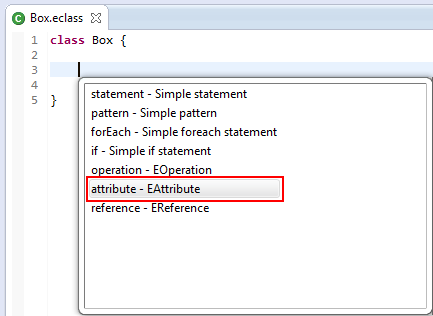
\includegraphics[width=0.5\textwidth]{eclipse_typeCompletion_main}
	\caption{eMoflon's type completion}
	\label{fig:typeComp_Main}
\end{figure} 

\item[$\blacktriangleright$] Type completion also supports you by providing a list of types. Start to create a second attribute, \texttt{stringRep}, but after
the \texttt{``:''} operator, press the same hotkeys. The new list provides all the types currently available - any further EClasses you create will also appear
in this list. Begin to type \texttt{EString} until the option is highlighted and press \texttt{enter} ({\bf get image}). Your workspace should now resemble
(Fig.~\ref{fig:boxDeclaration}).

\begin{figure}[h!]
	\centering
  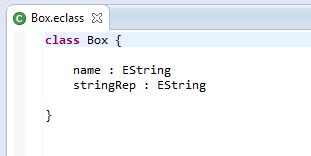
\includegraphics[width=0.5\textwidth]{eclipse_classBoxDeclaration}
	\caption{Newly created box class}
	\label{fig:boxDeclaration}
\end{figure} 
\FloatBarrier

\newpage

\item[$\blacktriangleright$] Now create two empty EClasses in your model, \texttt{Partition} and \texttt{Card}.

\item[$\blacktriangleright$] In \texttt{Partition}, add two \texttt{EInt} attributes, \texttt{index} and \texttt{partitionSize}.

\item[$\blacktriangleright$] In \texttt{Card}, create three \texttt{EString} attributes, \texttt{back}, \texttt{face} , and \texttt{partitionHistory}.

\item[$\blacktriangleright$] If you've done everything correctly, your workspace should now resemble Fig.~\ref{fig:workspaceClassAttributes}.

\vspace{0.5cm}

\begin{figure}[htbp]
	\centering
  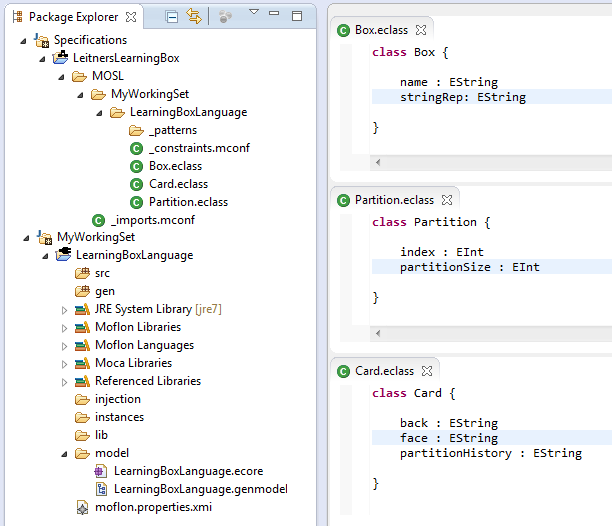
\includegraphics[width=1.0\textwidth]{eclipse_workspaceTexClassAttributes}
	\caption{Declaration of classes and attributes}
	\label{fig:workspaceClassAttributes}
\end{figure} 

\vspace{0.5cm}

\item[$\blacktriangleright$] That's it for declaring class attributes! Feel free to build your project again and view the changes in the \texttt{.ecore}
mode, and the generated files in ``gen" and ``src." On a final note, while some languages (such as Java) allow the declaration of several small classes (such as
these three) in the same file, when tooling with eMolfon, we keep them separated. Don't worry - we'll explain this later in the handbook. As for now, continue
to the next section to start creating references between these classes.

% \fancyfoot[R]{$\triangleright$ \hyperlink{static:references splash}{Next}}

\end{itemize}
